\graphicspath{{./fifth/img/}} % path to graphics

\section*{\LARGE Цель практической работы}
\addcontentsline{toc}{section}{Цель практической работы}

\textbf{Цель работы} --- сформировать навык построения диаграммы
деятельности в Visual Paradigm.
\textbf{Задачи}:
\begin{itemize}
	\item ознакомиться с назначением диаграммы деятельности и ее элементами;
	\item изучить возможности Visual Paradigm для построения
		диаграммы деятельности;
	\item построить диаграмму деятельности в Visual Paradigm
		в соответствии с предложенными заданиями.
\end{itemize}

\clearpage

\section*{\LARGE Выполнение практической работы}
\addcontentsline{toc}{section}{Выполнение практической работы}
\section{Создание диаграммы деятельности}
При модернизации шаблона следует добавить на диаграмму узел решения,
узел слияния, изменить узел разделения и узел соединения. Для получения
стрелок, идущих от элемента действия, к элементу решения (узел слияния),
следует использовать стрелку типа \textbf{Control Flow (CF)} Для получения
стрелок, изогнутых под углом 90 градусов, следует довести стрелку до места
изгиба, кликнуть левой кнопкой мышки и далее довести стрелку до нужного
элемента диаграммы. Диаграммы деятельности могут быть использованы для
моделирования бизнес-процессов. Применительно к бизнес-процессам
желательно выполнение каждого действия ассоциировать с конкретным
подразделением компании. В этом случае подразделение несет ответственность
за реализацию отдельных действий, а сам бизнес-процесс представляется в виде
переходов действий из одного подразделения к другому.\par
Для моделирования этих особенностей в языке UML используется
специальная конструкция, получившая название дорожки (swimlanes). При этом
все состояния действия на диаграмме деятельности делятся на отдельные
группы, которые отделяются друг от друга вертикальными линиями. Две
соседние линии и образуют дорожку, а группа состояний между этими линиями
выполняется отдельным подразделением.\par
Названия подразделений явно указываются в верхней части дорожки.
Пересекать линию дорожки могут только переходы, которые в этом случае
обозначают выход или вход потока управления в соответствующее
подразделение компании.\par
На рис. \ref{fig:activity} представлен пример диаграммы деятельности
с дорожками.

\begin{figure}[h!tp]
	\centering
	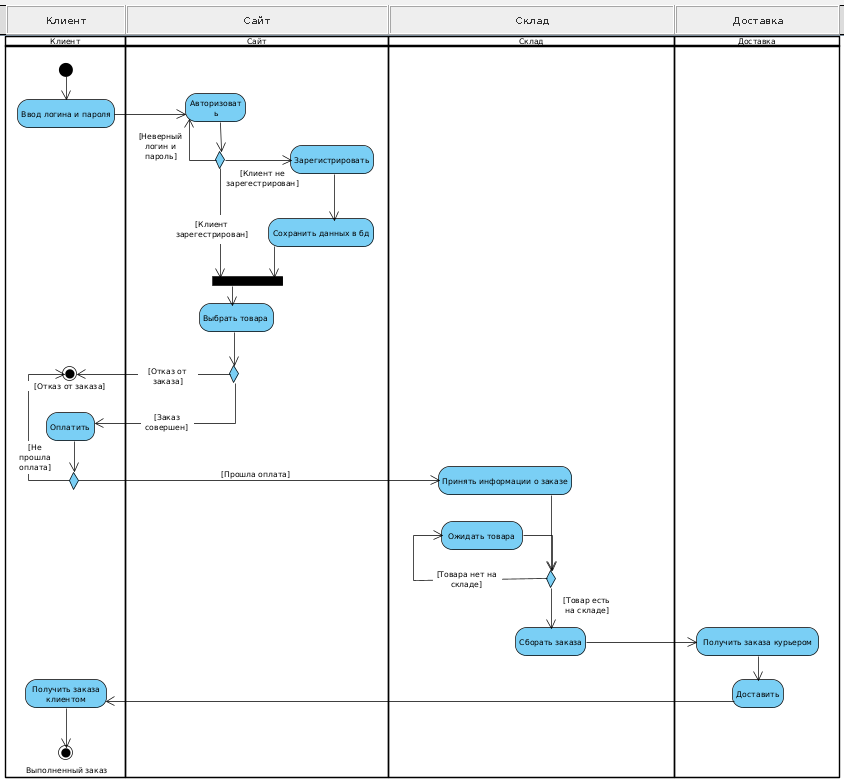
\includegraphics[width=1\textwidth]{Screenshot from 2023-04-19 13-16-26}
	\caption{Диаграмма деятельности с дорожками}
	\label{fig:activity}
\end{figure}


\clearpage

\section*{Ответы на вопросы}
\addcontentsline{toc}{section}{Ответы на вопросы}

\begin{description}
	\item [В чем состоит назначение диаграммы деятельности?]
		Для моделирования последовательности действий, которые выполняются
		различными элементами, входящими в состав системы.
	\item [Чем диаграммы деятельности отличаются от блок-схем? Какие
		преимущества это дает разработчикам?]
		Диаграмма деятельности отличается от традиционной блок-схемы
		\begin{itemize}
			\item более высоким уровнем абстракции
			\item возможностью представления с помощью диаграмм деятельности
				управления параллельными потоками наряду с последовательным
				управлением
		\end{itemize}
	\item [Какова роль диаграмм деятельности в проектировании
		информационных систем?]
		В уточнения вариантов использования и моделей последовательности.
	\item [Что описывает состояние деятельности на диаграмме деятельности?]
		Каждое состояние на диаграмме деятельности соответствует выполнению
		некоторой элементарной операции, а переход в следующее состояние
		срабатывает только при завершении этой операции
		в предыдущем состоянии.
	\item [В чем сходство и в чем отличия диаграмм состояний и деятельности?]
		Отличие заключается в семантике состояний, которые используются
		для представления не деятельностей, а действий, и в отсутствии на
		переходах сигнатуры событий. Каждое состояние на диаграмме
		деятельности соответствует выполнению некоторой элементарной операции,
		а переход в следующее состояние срабатывает только при завершении
		этой, операции в предыдущем состоянии.
	\item [С какими схемами, используемыми в структурном программировании,
		можно сравнить диаграмму деятельности?
		Что у них общего и в чем отличия?]
		Диаграммы деятельности могут быть сравнены с блок-схемами,
		используемыми в структурном программировании. Общим между ними
		является то, что они обе визуализируют последовательность выполнения
		операций в системе, задания и условия выбора. \par
		Однако есть и различия между диаграммами деятельности и блок-схемами.
		В отличие от блок-схем, диаграммы деятельности могут использоваться
		для описания более сложных процессов, которые могут включать
		не только линейный, но и параллельный, циклический и условный ход
		выполнения операций. Диаграммы деятельности позволяют описывать
		действия и принимаемые решения на каждом этапе выполнения процессов,
		а также их связи с другими процессами.
	\item [Каким образом на диаграмме деятельности отображается
		разветвление процесса?]
		С помощью узлов: решения (decision node), слияния (merge note),
		разделения (fork node), соединения (join node).
	\item [Для чего на диаграмме деятельности используется элемент
		«Дорожка»?]
		Когда, например в бизнес-процессах, желательно выполнение каждого
		действия ассоциировать с конкретным подразделением компании.
	\item [Каковы правила и рекомендации при построении диаграммы
		деятельности?]
		Правила и рекомендации:
		\begin{enumerate}
			\item При построении диаграмм рекомендуется использовать
				классические принципы моделирования.
			\item Количество пересечений линий следует минимизировать.
			\item Если на диаграмме имеется ветвление/решение на параллельные
				или альтернативные потоки, то должно указываться
				и соответствующее соединение/слияние этих потоков.
			\item В целях определения зоны ответственности (набора действий)
				сущностей рекомендуется использовать разделы деятельности.
			\item В одно действие может входить только один поток управления.
		\end{enumerate}
	\item [Как моделируются начальное и конечное состояния?]
		С помощью начального узела (initial node) и узла финала деятельности.
	\item [Как обозначают на диаграмме точку принятия решения? Когда
		нужно моделировать принятия решений?]
		Точка принятия решения на диаграмме деятельности обычно обозначается
		ромбом с текстом внутри, который описывает условие принятия решения.
		Элемент, который обозначает точку принятия решения, имеет один вход
		и два или более выхода, в зависимости от количества возможных исходов
		для принятия решения.\par
		Принятие решения моделируется на диаграмме деятельности, когда на
		выполнение процесса влияют различные условия и требуются решения для
		выбора одного или нескольких путей выполнения.
\end{description}

\clearpage

\section*{\LARGE Вывод}
\addcontentsline{toc}{section}{Вывод}
Мы создали диаграмму активности.
При этом были использованы классические
принципы моделирования --- декомпозиции и иерархического упорядочения.
Также учли, что потоки данных или управления в местах пересечений не
меняют своего направления. И опередлили зоны ответственности сущностей.

